\documentclass[11pt]{article}
\usepackage{fancyhdr}  % For headers and footers
\usepackage[margin=1in]{geometry}  % Set margins
\usepackage{tcolorbox}  % For creating the double-lined box
\usepackage{graphicx}   % For extending lines within margins
\usepackage{amsmath}
\usepackage{amssymb}
\usepackage{amsthm}
\usepackage{enumitem}
\usepackage{lastpage}
\usepackage{array}
\usepackage{booktabs}
\usepackage{pgfplots}
\usepackage{tikz}
\usepackage{hyperref}
\usepackage{xcolor}
\usepackage{mdframed}
\usepackage{booktabs}

\definecolor{horange}{HTML}{f58026}

\hypersetup{
	colorlinks=true,
	linkcolor=horange,
	filecolor=horange,      
	urlcolor=horange,
}

\setlist[enumerate]{left=0.2cm}

% Need to add in customization for examples
\newcommand{\sol}[1]{
    \begin{customframedproof}
        \begin{solution}
        #1
        \end{solution}
    \end{customframedproof}
}

\newmdenv[
  topline=false,
  bottomline=false,
  rightline=false,
  leftline=true,
  linewidth=1.5pt,
  linecolor=black!45, % default color, will be overridden in custom commands
  innertopmargin=0pt,
  innerbottommargin=0pt,
  innerrightmargin=10pt,
  innerleftmargin=10pt,
  leftmargin=0pt,
  rightmargin=0pt,
  skipabove=\topsep,
  skipbelow=\topsep,
]{customframedproof}

\newenvironment{solution}
  {\textit{Solution.}}

  % Command for theorems proofs with a predefined color
\newcommand{\pf}[1]{
    \begin{customframedproof}
        \begin{proof}
        #1
        \end{proof}
    \end{customframedproof}
}


% Header formatting for all pages except the title page
\fancypagestyle{standard}{
    \fancyhf{}
    \fancyhead[L]{Exam I -- Take Home}
    \fancyhead[R]{Cryptography}
    \fancyfoot[R]{\rule{\textwidth}{0.5pt} \\ Page \thepage\ of \pageref*{LastPage}} % Right-aligned footer with page numbers
}

\newcommand{\points}[1]{\marginpar{[#1]}} % Define a command for margin points

% Header formatting for the title page
\fancypagestyle{titlepage}{
    \fancyhf{}
    \fancyhead[L]{Hendrix}
    \fancyhead[C]{Sept. 19, 2024}  % Centered date in title page header
    \fancyhead[R]{Mathematical Cryptography}
}

\setlength{\footskip}{0in}

% Natural Numbers 
\newcommand{\N}{\mathbb{N}}

% Whole Numbers
\newcommand{\W}{\mathbb{W}}

% Integers
\newcommand{\Z}{\mathbb{Z}}

% Rational Numbers
\newcommand{\Q}{\mathbb{Q}}

% Real Numbers
\newcommand{\R}{\mathbb{R}}

% Complex Numbers
\newcommand{\C}{\mathbb{C}}

\linespread{1}

\pgfplotsset{compat=1.18}

\begin{document}

% Title page
\thispagestyle{titlepage}

\begin{center}
    {\large Exam 1 -- Take home}
\end{center}

\noindent Printed Name: Paul Beggs \underline{\hspace{341.49907pt}}



\begin{center}
    \fbox{%
        \fbox{%
            \parbox{15.2cm}{%
                \textbf{Instructions:} This is an individual, open-book, open-notes exam. You may not give help, receive help, or discuss this exam with anyone apart from me. \\

                You may use a calculator or the computer to help with computations, just be sure to cite when you do so. \\

                You may consult your textbook, your personal class notes, and your previous homework assignments while working on this exam. You may also consult anything posted on our Teams page. Only these resources are allowed. \\

                You may NOT consult any other sources. No internet sources. No other textbooks. No notes or any other material from other students. No consulting with another student. No consulting with another professor. \\

                As always, show work to get full credit (the correct answer may NOT be enough). \\
                Write clearly! Double check your answers! \\

                \textbf{Honor Pledge: I have neither received nor given aid on this work, nor have I witnessed any such violation of the Honor Code.}\\

                \textbf{Honor Pledge Signature:}\underline{\hspace{299.05994pt}}
                \vspace{0.00001cm}
            }%
        }%
    }%
\end{center}
\vspace{0.9cm}
\begin{table}[h]
    \centering
    \renewcommand{\arraystretch}{1.5} % Increase row height
    \begin{tabular}{ccc}
        \toprule
        Question & Points & Score \\ \midrule
        1        & 10     &       \\ \midrule
        2        & 10     &       \\ \midrule
        3        & 10     &       \\ \midrule
        Total:   & 30     &       \\ \bottomrule
    \end{tabular}
\end{table}

\vfill

\newpage



% Following pages use the standard header
\pagestyle{standard}
\begin{enumerate}

    \item Let \(a,b\) be positive integers and \(D = \gcd(a,b)\). Prove that if \(x^a \equiv 1 \ (\text{mod } m)\) and\points{10} \\
          \(x^b \equiv 1 \ (\text{mod } m)\) then \(x^D \equiv 1 \ (\text{mod } m)\). \\

          \textbf{Definitions to be used in the proof:}
          \begin{enumerate}
              \item \textbf{Divides:} For integers \(a,b \in \Z\), we say that \(a\) divides \(b\) if there exists an integer \(c\) such that \(b = ac\). Notated as \(a \mid b\).
              \item \textbf{GCD:} The greatest common divisor of two integers \(a\) and \(b\), denoted \(D = \gcd(a,b)\), is the largest positive integer such that \(D \mid a\) and \(D \mid b\). This means there exists \(p,q \in \Z\) such that \(D = pa + qb\).
          \end{enumerate}
          \pf{
              Let \(a,b\) be positive integers and \(D = \gcd(a,b)\), and suppose \(x^a \equiv 1 \ (\text{mod } m)\) and \(x^b \equiv 1 \ (\text{mod } m)\). Since \(D = \gcd(a,b)\), we know that there exists \(p,q \in \Z\) such that \(D = pa + qb\) by the definition of GCD. Now, consider \(x^D \equiv 1 \ (\text{mod } m)\). We can rewrite \(x^D\) as \(x^{pa + qb}\), and apply the properties of exponents. This gives us \(x^{pa + qb} = (x^a)^p \cdot (x^b)^q\). Since \(x^a \equiv 1 \ (\text{mod } m)\) and \(x^b \equiv 1 \ (\text{mod } m)\), we can substitute these values into the equation. This gives us \((x^a)^p \cdot (x^b)^q = 1^p \cdot 1^q = 1\). Therefore, \(x^D \equiv 1 \ (\text{mod } m)\).
          }

          \newpage
          \pagestyle{standard}

    \item Prove that the set \(\mathbb{Q}\) of rational numbers is a ring under addition and multiplication. Remember\points{10} that you are only allowed to assume knowledge of the properties of integers, so treat \(\mathbb{Q}\) as the set \(\displaystyle \mathbb{Q} = \left\{ \frac{a}{b} \ \Big| \ a,b \in \mathbb{Z} \text{ and } b \ne 0 \right\} \). \\
          \pf{
              For the following, let \(x = \frac{a}{b}\), \(y = \frac{c}{d}\), and \(z = \frac{e}{f}\) be rational numbers in \(\Q\) such that \(a,b,c,d,e,f \in \Z\) where \(b,d,f \ne 0\). We want to show that the set \(\mathbb{Q}\) of rational numbers is a ring under addition and multiplication. Thus, consider the following:
              \begin{enumerate}
                  \item \textbf{Additive Closure.} \\
                        Consider \(\frac{ad + bc}{bd}\). Since \(a,b,c,d \in \Z\), we know that \(ad + bc \in \Z\) because integer addition is closed. Moreover, because \(b,d \ne 0\), we know that \(bd \ne 0\). Therefore, \(\frac{ad + bc}{bd} \in \Q\). This shows that rational numbers are closed under addition.
                  \item \textbf{Additive Associativity.} \\
                        Consider \((x + y) + z = (\frac{a}{b} + \frac{c}{d}) + \frac{e}{f} = \frac{ad + bc}{bd} + \frac{e}{f} = \frac{(ad + bc)f + edb}{bdf}\) because we know that the integers possess distributivity we know that  \(\frac{(ad + bc)f + edb}{bdf} = \frac{adf + bcf + cdb}{bdf}\). Similarly, consider \(x + (y + z) = \frac{a}{b} + (\frac{c}{d} + \frac{e}{f}) = \frac{a}{b} + \frac{cf + ed}{df} = \frac{a(df) + (cf + ed)b}{bdf} = \frac{adf + cbf + ebd}{bdf}\). By substitution, we can see that \((x + y) + z = x + (y + z)\). This shows that rational numbers are associative under addition.
                  \item \textbf{Additive Commutativity.} \\
                        Consider \(x + y = \frac{a}{b} + \frac{c}{d} = \frac{ad + cb}{bd}\). Then, consider \(y + x = \frac{c}{d} + \frac{a}{b} = \frac{cb + ad}{db}\). Because addition is commutative in the integers, we know that \(ad + cb = cb + ad\). Therefore, \(x + y = y + x\). This shows that rational numbers are commutative under addition.
                  \item \textbf{Additive Identity.} \\
                        Let \(0 := \frac{0}{1}\). Consider \(x + 0 = \frac{a}{b} + \frac{0}{1} = \frac{a \cdot 1 + 0 \cdot b}{b \cdot 1} = \frac{a}{b}\). This shows that the additive identity is 0.
                  \item \textbf{Additive Inverse.} \\
                        Let \(-x := \frac{-a}{b}\). Consider \(x + (-x) = \frac{a}{b} + \frac{-a}{b} = \frac{a \cdot b + -a \cdot b}{b \cdot b} = \frac{0}{b^2} = 0\). This shows that the additive inverse is \(-x\).
                  \item \textbf{Multiplicative Closure.} \\
                        Consider \(x \cdot y = \frac{ac}{bd}\). Since \(a,b,c,d \in \Z\), we know that \(ac \in \Z\) because integer multiplication is closed. Moreover, because \(b,d \ne 0\), we know that \(bd \ne 0\). Therefore, \(\frac{ac}{bd} \in \Q\). This shows that rational numbers are closed under multiplication.
                  \item \textbf{Multiplicative Associativity} \\
                        Consider \((x \cdot y) \cdot z = (\frac{a}{b} \cdot \frac{c}{d}) \cdot \frac{e}{f} = \frac{ac}{bd} \cdot \frac{e}{f} = \frac{ace}{bdf}\). Similarly, consider \(x \cdot (y \cdot z) = \frac{a}{b} \cdot (\frac{c}{d} \cdot \frac{e}{f}) = \frac{a}{b} \cdot \frac{ce}{df} = \frac{ace}{bdf}\). By substitution, we can see that \((x \cdot y) \cdot z = x \cdot (y \cdot z)\). This shows that rational numbers are associative under multiplication.
                  \item \textbf{Distributive Property.} \\
                        Consider \(x \cdot (y + z) = \frac{a}{b} \cdot (\frac{c}{d} + \frac{e}{f}) = \frac{a}{b} \cdot \frac{cf + ed}{df} = \frac{acf + aed}{bdf}\). Similarly, consider \(x \cdot y + x \cdot z = \frac{a}{b} \cdot \frac{c}{d} + \frac{a}{b} \cdot \frac{e}{f} = \frac{ac}{bd} + \frac{ae}{bf} = \frac{acf + aed}{bdf}\). By substitution, we can see that \(x \cdot (y + z) = x \cdot y + x \cdot z\). This shows that rational numbers are distributive under multiplication.\qedhere
              \end{enumerate}
          }


          \newpage
          \pagestyle{standard}

    \item The following is the full message that was encrypted using the monoalphabetic cipher mentioned\points{10} on the in-class exam. Use \hyperlink{Plot_1}{Plot 1} and \hyperlink{Plot_2}{Plot 2} to decrypt the following message and include notes along the way on your thought process (why you made certain choices, why something did or did not seem to work, etc.)

          \begin{center}
              \fontsize{14}{16}\selectfont % Set font size to 14pt
              \begin{tabular}{llllllll}
                  \texttt{JMAVE} & \texttt{EOMKE} & \texttt{LEKEK} & \texttt{VMREE} & \texttt{NJMAV} & \texttt{EEOMK} & \texttt{ELEKE} & \texttt{KVMRE} \\
                  \texttt{ENSNK} & \texttt{VSOQM} & \texttt{AXQMX} & \texttt{NQQEK} & \texttt{VMEKV} & \texttt{MYKVS} & \texttt{NLONE} & \texttt{KDMAX} \\
                  \texttt{IOMKV} & \texttt{MBXYM} & \texttt{MXOBD} & \texttt{IKDMA} & \texttt{XIOMK} & \texttt{VMBXY} & \texttt{MVXYQ} & \texttt{DMAXI} \\
                  \texttt{OMKVX} & \texttt{KLEXP} & \texttt{JSPPO} & \texttt{MYHMK} & \texttt{EEYLX} & \texttt{NSZMX} & \texttt{NQRMX} & \texttt{DIYMK} \\
                  \texttt{VMDMO} & \texttt{KEFEI} & \texttt{YMNMY} & \texttt{LSMOX} & \texttt{NQOCS} & \texttt{PPODM} & \texttt{AXIOM} & \texttt{KVXKA} \\
                  \texttt{VXPPM} & \texttt{NLMSO} & \texttt{ENMKV} & \texttt{XKJMX} & \texttt{YMJSP} & \texttt{PSNLK} & \texttt{EXAAM} & \texttt{WKENM} \\
                  \texttt{JMXYM} & \texttt{INJSP} & \texttt{PSNLK} & \texttt{EWEOK} & \texttt{WENMX} & \texttt{NQENM} & \texttt{JVSAV} & \texttt{JMSNK} \\
                  \texttt{MNQKE} & \texttt{JSNXN} & \texttt{QKVME} & \texttt{KVMYO} & \texttt{KEE}
              \end{tabular}
          \end{center}

          \sol{
              \begin{enumerate}
                  \item I substituted varying letters that are common in English for the most common letters in the ciphertext. For example, I substituted the letter \texttt{M} for the letter \texttt{E} since \texttt{M} is the most common letter in the ciphertext. I also substituted the letter \texttt{K} for the letter \texttt{T} since \texttt{V} is the second most common letter in the ciphertext. I continued this process until I got a string of letters that did not make sense together.
                  \item When I would eventually run into problems with the mismatched string of characters, I would try to match letters that may fit into both the monogram frequency and the bigram frequency. This influenced my thoughts on whether \texttt{M} was \texttt{T} or \texttt{E}.
                  \item Once most of the substitutions were made and there were still some characters that were out of place, I would reconsider a selection for a substitution that I made for one that made more sense.
                  \item I would iterate over this list until all the words made sense together.
              \end{enumerate}

              \textbf{Decrypted text:} \\
              We choose to go to the moon. We choose to go to the moon in this decade and do the other things, not
              because they are easy, but because they are hard, because that goal will serve to organize and
              measure the best of our energies and skills, because that challenge is one that we are willing to accept, one we are unwilling to postpone, and one which we intend to win, and the others, too.
          }

\end{enumerate}

\newpage
\begin{center}
    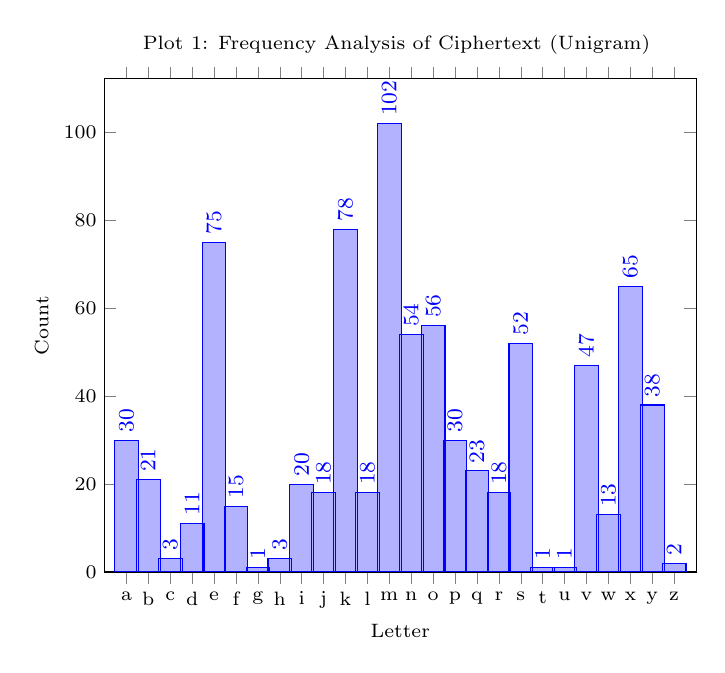
\begin{tikzpicture}
        \scriptsize
        \begin{axis}[width=0.75\linewidth,
                ybar = 1mm,
                bar width = 3mm,
                enlarge x limits=0.04,
                ylabel={Count},
                xlabel={Letter},
                title={Plot 1: Frequency Analysis of Ciphertext (Unigram) \label{Plot_1}},
                symbolic x coords={a,b,c,d,e,f,g,h,i,j,k,l,m,n,o,p,q,r,s,t,u,v,w,x,y,z},
                xtick=data,
                ymin=0,
                nodes near coords,
                nodes near coords style={rotate=90, anchor=west, font=\footnotesize},
            ]
            \addplot coordinates {
                    (a, 30)
                    (b, 21)
                    (c, 3)
                    (d, 11)
                    (e, 75)
                    (f, 15)
                    (g, 1)
                    (h, 3)
                    (i, 20)
                    (j, 18)
                    (k, 78)
                    (l, 18)
                    (m, 102)
                    (n, 54)
                    (o, 56)
                    (p, 30)
                    (q, 23)
                    (r, 18)
                    (s, 52)
                    (t, 1)
                    (u, 1)
                    (v, 47)
                    (w, 13)
                    (x, 65)
                    (y, 38)
                    (z, 2)
                };
        \end{axis}

    \end{tikzpicture} \\
\end{center}

\begin{center}
    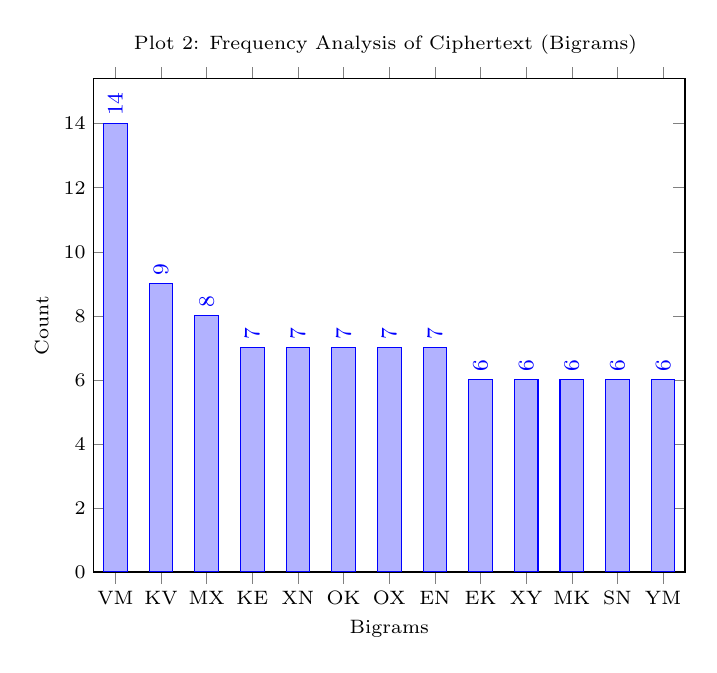
\begin{tikzpicture}
        \scriptsize
        \begin{axis}[width=0.75\linewidth,
                ybar = 1mm,
                bar width = 3mm,
                enlarge x limits=0.04,
                ylabel={Count},
                xlabel={Bigrams},
                title={Plot 2: Frequency Analysis of Ciphertext (Bigrams) \label{Plot_2}},
                symbolic x coords={VM,KV,MX,KE,XN,OK,OX,EN,EK,XY,MK,SN,YM},
                xtick=data,
                ymin=0,
                nodes near coords,
                nodes near coords style={rotate=90, anchor=west, font=\footnotesize},
            ]
            \addplot coordinates {
                    (VM, 14)
                    (KV, 9)
                    (MX, 8)
                    (KE, 7)
                    (XN, 7)
                    (OK, 7)
                    (OX, 7)
                    (EN, 7)
                    (EK, 6)
                    (XY, 6)
                    (MK, 6)
                    (SN, 6)
                    (YM, 6)
                };
        \end{axis}
        \label{Plot_2}  % Moved here
    \end{tikzpicture} \\
\end{center}

Graph from \href{https://tex.stackexchange.com/questions/610173/pgf-plot-for-frequency-analysis}{this link}.



\end{document}